\section{The Ceiling Speed Monitoring Function -- Functional Objectives}
\label{sec:ceil}
% ======================================================================
 
The
European Train Control System ETCS relies on the existence of an onboard controller
in train engines, the \emph{European Vital Computer EVC}. Its functionality and basic architectural features are described in the public ETCS system specification~\cite{ETCS}. 
One functional category of the EVC covers aspects of speed and distance monitoring, to accomplish the  \emph{``\ldots supervision of the speed of the train versus its position, in order to assure that the train remains within the given speed and distance limits.''}~\cite[3.13.1.1]{ETCSSRS-Principles}. Speed and distance monitoring  is decomposed into three sub-functions~\cite[3.13.10.1.2]{ETCSSRS-Principles}, where only one out of these three is active at a point in time:
\begin{enumerate}
\item \emph{Ceiling speed monitoring (CSM)} supervises the observance of the maximal speed allowed according to the current most restrictive speed profile (MRSP). CSM is active while the train does not approach a target (train station, level crossing, or any other   point that must be reached with predefined speed).

\item \emph{Target speed monitoring (TSM)} supervises the observance of the maximal distance-depending  speed, while the train brakes to a target, that is, a location where a given predefined speed (zero or greater zero) must be met.

\item \emph{Release speed monitoring (RSM)} applies when the special target ``end of movement authority (EOA)'' is approached, where the train must come to a stop. RSM supervises the observance of the distance-depending  so-called release speed, when the train approaches the EOA. 
\end{enumerate}

In this technical report we present a complete formal model of the CSM function, with the objective to derive a complete test suite from this model (Section~\ref{sec:iecpstart}).


% ----------------------------------------------------------------------
\section{Model Description}\label{sec:modeldesc}


% .......................................................................
\subsection{Model Availability} 


The ceiling speed monitor has been modelled using the {\it OMG Systems Modeling Language (OMG SysML$^{TM}$)}~\cite{SysML12}. 
The complete   model   is available for download under {\tt http://www.mbt-benchmarks.org}. This is a website dedicated to the publication of test models possessing features that are of general interest for researchers and practitioners in the field of model-based testing (MBT). Moreover, the models may serve as benchmarks for comparing test automation tools with respect to test strength and tool performance. This has been further motivated in~\cite{pel2011a}, where also suggestions for MBT benchmarks are given.
In this section, we give a comprehensive introduction into the formal model.


% .......................................................................
\subsection{Model Components} 

According to the model-based testing approach applied in this report, UML/SysML test models are 
structured into the following basic components.
\begin{enumerate}
\item A package containing the system requirements (Fig.~\ref{fig:req}),
\item A block diagram  (Fig.~\ref{fig:sysif}) identifying 
\begin{itemize}
\item the system under test (SUT),
\item its interface to the operational environment, and
\item the test environment (TE) simulating the ``real'' operational environment during test execution,
\end{itemize}
\item Subordinate block diagrams refining the internal structure of the SUT (Fig.~\ref{fig:sutcomposite}) and the TE, respectively, 
\item State machines associated with the leaf blocks of the structural decompositions of SUT (Fig.~\ref{fig:csmsmtl}) and TE, and
\item Operations associated with blocks. These are referenced by state machines, when evaluating guard conditions or performing actions.
\end{enumerate}



% .......................................................................
\subsection{Model Semantics -- Overview} 

The detailed formal behavioural semantics of SysML test models has been described 
in~\cite[pp.~88]{d341}. This semantics is consistent with the
standards~\cite{uml_2_4,SysML12}, but fixes certain semantic variation points in
 ways that are admissible according to the standards.
In this technical report, however, the semantic details will be explained as far as they are relevant for understanding the model presented here: in the present section, the behavioural   semantics of the CSM model is 
informally explained, and in Section~\ref{sec:transrel}, the formal model semantics is specified by presenting its transition relation. 

The leaf components of the structural model decomposition execute concurrently. For the model under consideration the SUT operates in a sequential manner, but concurrently with its environment. In this test model, the  behaviour of the TE is undetermined; this is interpreted in the way that every possible sequence of input vectors to the SUT would be allowed.  This assumption is reasonable for the example considered here: due to robustness requirements, the ceiling speed monitor must be able to cope with input sequences that may be unreasonable from a physical point of view. TE components are  introduced in situations where only certain types of interactions between operational environment and SUT are possible.  

The model executes according to the {\it run-to-completion} semantics defined 
for state machines in~\cite{uml_2_4}. The model is in a {\it quiescent} (or stable) state, if 
no transition can be executed without an input change. In a quiescent model state, inputs may be changed. If these changes enable a transition, the latter is executed. Since our SUT model is deterministic -- this is typical for safety-relevant applications -- there is no necessity to handle   situations where several transitions are simultaneously enabled. The executed transition, however, may lead to a {\it transient} state, that is, to a state where another transition is enabled. In the run-to-completion semantics this new transition is also executed, and so forth until a quiescent state is reached. Conceptually, the consecutive execution of model transitions is executed in zero time, so that input changes cannot happen until the next quiescent state has been reached. Moreover, models admitting unbounded sequences of transitions between transient states are considered as illegal, and this situation is called a {\it livelock} failure.



% .......................................................................
\subsection{Interfaces}

The interfaces between SUT and its environment are specified in the
internal block diagram displayed in Fig.~\ref{fig:sysif}. All
interfaces are represented as flow ports. The environment writes to
SUT input ports and reads from SUT output ports.

 \begin{figure}
 %%\hspace*{-40mm}
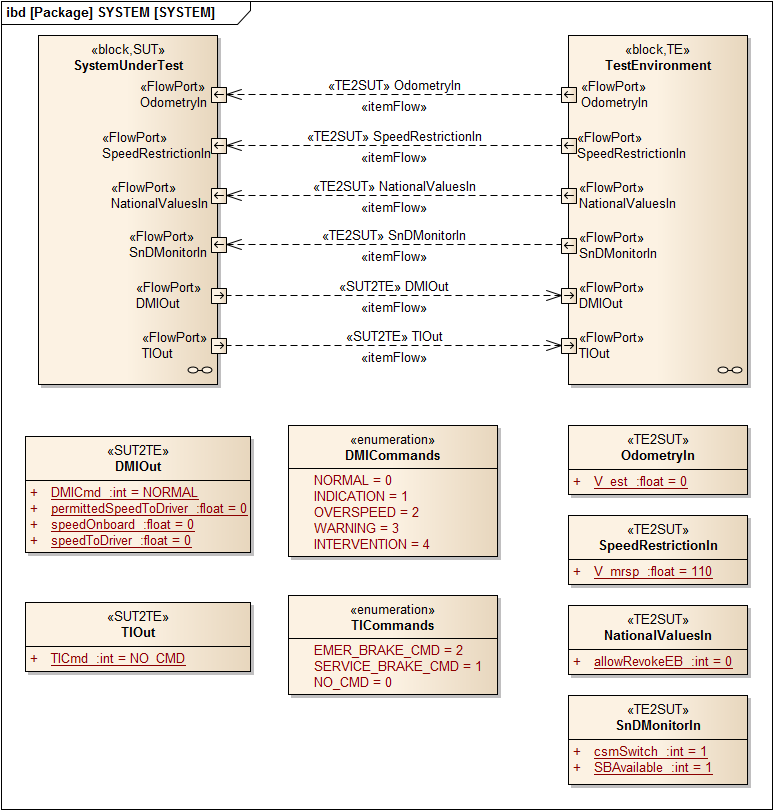
\includegraphics[width=\textwidth]{SYSTEM_INTERFACE.png}
%%\vspace*{-35mm}
\caption{System interface of the ceiling speed monitor.}
 \label{fig:sysif}
 \end{figure}
 
Ceiling speed monitoring is activated and de-activated by the speed and distance monitoring (SnD) coordination function that controls CSM, TSM, and RSM: on input interface {\sf SnDMonitorIn}, variable  $\csmsw$   specifies whether ceiling speed monitoring should be active ($\csmsw=1$) or passive, since target  or release speed monitoring is being performed ($\csmsw = 0$). Furthermore, this interface carries variable $\sbia$ which has value 1, if the train is equipped with a service brake. This brake is then used for slowing down the train if it has exceeded the maximal speed allowed, but not yet reached the threshold for an emergency brake intervention. If $\sbia = 0$, the emergency brake shall be used for slowing down the train in this situation. Input $\sbia$ is to be considered as  a configuration parameter of the train, since it depends on the availability of the service brake hardware. Therefore this value can be freely selected at start-of-test, but must remain constant during test execution.



Input interface {\sf OdometryIn} provides the current speed value
estimated by the odometer equipment in variable $\vest$. Input
interface {\sf SpeedRestrictionIn} provides the current maximal
velocity defined by the most restrictive speed profile in variable
$\vmax$. Input interface {\sf NationalValuesIn} provides a control
flag for the ceiling speed monitor: variable $\text{allowRevokeEB}$ is
1, if after an emergency brake intervention the brake may be
automatically released as soon as the estimated velocity of the train
is again less or equal to the maximal speed allowed. Otherwise
($\text{allowRevokeEB} = 0$) the emergency brakes must only be
released after the train has come to a standstill ($\vest = 0$).
This input parameter is called a ``national value'', because it may change when a
train crosses the boundaries between European countries, due to their local regulations.


Output interface {\sf DMIOut} sends data from the SUT to the driver
machine interface (DMI). It carries five variables. $\dmicmd$ is used
to display the supervision status to the train engine driver: Value
INDICATION may be initially present when CSM is activated, but will be
immediately overridden by one of the values NORMAL, OVERSPEED,
WARNING, or INTERVENTION, as soon as ceiling speed monitoring becomes
active. Value NORMAL is written by the SUT to this variable as long as
the ceiling speed is not violated by the current estimated
speed. Value OVERSPEED has to be set by the CSM as soon as condition
$\vmax < \vest$ becomes true. If the speed increases further (the
detailed conditions are described below), the indication changes from
OVERSPEED to WARNING, and from there to INTERVENTION. The latter value
indicates that either the train is slowed down until it is back in the
normal speed range, or the emergency brake has been triggered to stop
the train.  Furthermore, interface {\sf DMIOut} contains the following 
speed-related variables that are displayed as y/t-diagrams on the DMI.
\begin{itemize}
\item $\std$: the current estimated speed as given by variable $\vest$.
\item $\pstd$: the permitted maximal speed as given by the most 
restrictive speed profile $\vmax$.
\item $\sob$: maximal speed allowed ($\vmax$) as long as the train does not
overspeed.  Otherwise it carries values $\vmax + \delta$, where
$\delta > 0$ specifies the margin from $\vmax$ to service brake
intervention and is calculated as described below.  
\end{itemize}




Output interface {\sf TIout} specifies the train interface from the CSM to the brakes, using 
variable $\text{TICmd}$. If $\text{TICmd} = \text{NO\_CMD}$, both service brakes (if existent) and
emergency brakes are released. If $\text{TICmd} = \text{SERVICE\_BRAKE\_CMD}$, the service brake 
is activated. If $\text{TICmd} = \text{EMER\_BRAKE\_CMD}$, the emergency brake is triggered.



% .......................................................................
\subsection{SUT Attributes and Operations}\label{sec:ops}
The CSM is modelled as an application with sequential behaviour. Therefore the 
SUT block on the top-level interface diagram (Fig.~\ref{fig:sysif})  is refined into another block 
diagram that just carries the SUT, as shown in Fig.~\ref{fig:sutcomposite}.




 \begin{figure}[htbp]
%\hspace*{-50mm}
\centering
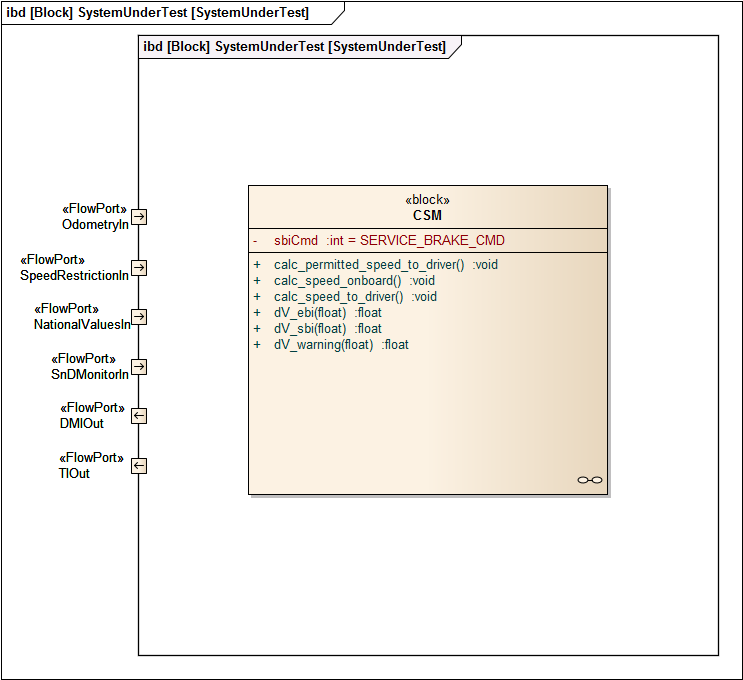
\includegraphics[width=1\textwidth]{SystemUnderTest.png}
%%\vspace*{-35mm}
\caption{Block diagram with CSM (sequential behaviour).}
 \label{fig:sutcomposite}
 \end{figure}



As shown there, the SUT uses a local attribute $\sbicmd$ which 
carries value SERVICE\_BRAKE\_CMD, if the service
brake should be used for slowing down the train to the admissible
speed. If the value EMER\_BRAKE\_CMD is assigned to 
$\sbicmd$, the emergency brake will be triggered in this situation.

Operations $\calcw, \calcs, \calce$ return values that are used to
determine whether a warning should be indicated to the train engine
driver ($\vest > \vmax+\dvw(\vmax)$), a service brake intervention should be
triggered ($\vest > \vmax+\dvs(\vmax)$), or the emergency brake should be
activated ($\vest > \vmax+\dve(\vmax)$).  In each case, the calculation is performed
according to the pattern
\begin{equation}\label{eq:dvcalc}
\text{dV}_x(\vmax) = \left\{
\begin{array}{l}
\min\{\text{dV}_{x\text{min}} + C_x\cdot(\vmax-\text{V}_{x\text{min}}) ,\text{dV}_{x\text{max}} \}  \\\tabh   \text{if}\ \ \vmax > \text{V}_{x\text{min}} \\
\text{dV}_{x\text{min}}  
\\\tabh    \text{if}\ \ \vmax\le  \text{V}_{x\text{min}} \\
\end{array}
\right.
\end{equation}
which has been defined in~\cite[3.13.9.2.3]{ETCSSRS-Principles}. Here $x$ can be replaced by {\sf warning}, {\sf sbi} (SBI = service brake intervention), and {\sf ebi} (EBI = Emergency Brake Intervention), and $C_x$ is defined by 
$$
C_x = \frac{\text{dV}_{x\text{max}} - \text{dV}_{x\text{min}}}{\text{V}_{x\text{max}} - \text{V}_{x\text{min}}}
$$
The following minimal and maximal values apply~\cite[A.3.1]{ETCSSRS-Principles}:

\begin{center}
\bigskip
\begin{tabular}{|l|l|l|}\hline\hline
$\text{dV}_{\mathsf{warning}\text{min}} = 4$ & $\text{dV}_{\mathsf{sbi}\text{min}} = 5.5$ &  $\text{dV}_{\mathsf{ebi}\text{min}} =  7.5$
\\\hline
$\text{dV}_{\mathsf{warning}\text{max}} = 5$ & $\text{dV}_{\mathsf{sbi}\text{max}} = 10$ &  $\text{dV}_{\mathsf{ebi}\text{max}} = 15$
\\\hline\hline
$\text{V}_{\mathsf{warning}\text{min}} = 110$ & $\text{V}_{\mathsf{sbi}\text{min}} = 110$ &  $\text{V}_{\mathsf{ebi}\text{min}} =  110$
\\\hline
$\text{V}_{\mathsf{warning}\text{max}} = 140$ & $\text{V}_{\mathsf{sbi}\text{max}} = 210$ &  $\text{V}_{\mathsf{ebi}\text{max}} = 210$
\\\hline
\hline
\end{tabular}
\end{center}
Inserting these values into Equation~(\ref{eq:dvcalc}) results in
\begin{equation}\label{eq:dvw}
\dvw(\vmax) = \left\{
\begin{array}{lc}
\min\{\frac{1}{3} + \frac{1}{30}\cdot\vmax,5 \}  &    \text{if}\ \ \vmax > 110 \\
4  &  \text{if}\ \ \vmax\le  110 \\
\end{array}
\right.
\end{equation}

\begin{equation}\label{eq:dvsbi}
\dvs(\vmax) = \left\{
\begin{array}{lc}
\min\{0.55+0.045\cdot\vmax,10 \}  &    \text{if}\ \ \vmax > 110 \\
5.5  &  \text{if}\ \ \vmax\le  110 \\
\end{array}
\right.
\end{equation}

\begin{equation}\label{eq:dvwe}
\dve(\vmax) = \left\{
\begin{array}{lc}
\min\{-0.75 + 0.075\cdot\vmax,15 \}  &    \text{if}\ \ \vmax > 110 \\
7.5  &  \text{if}\ \ \vmax\le  110 \\
\end{array}
\right.
\end{equation}

Operations $\calcstd$ and $\calcpstd$ support the display of the current estimated
speed and the maximum speed, respectively, at the driver machine interface by performing assignments to output variables:
\begin{align*}
\std &= \vest\\
\pstd &= \vmax
\end{align*}


Operation $\calcsob$ displays the maximal speed $\vmax$ specified by the most restrictive speed profile in DMI interface variable $\sob$, as long  as the train is not overspeeding. As soon as $\vest > \vmax$, this function calculates the service brake intervention speed and displays it
via  $\sob$, that is,
$$
   \sob = \vmax + \dvs(\vmax)
$$
where $\dvs(\vmax)$ is calculated according to Equation~\ref{eq:dvsbi}.

% .......................................................................
%\newpage
\subsection{Requirements}\label{sec:req}
Figure~\ref{fig:req} shows the requirements reflected by the model.
The requirement labels refer to the sections of the ETCS standard document~\cite{ETCSSRS-Principles}, from where they have been imported into the model. To make   this technical report sufficiently self-contained, we list the requirements applicable to CSM in Table~\ref{tab:req}, and adapt the wording and the cross references to the technical report.

 
In requirement REQ-3.13.10.2.2, the traction cut-off command on the train interface is not explicitly addressed in our model, because it will always be triggered in synchrony with a braking command. We assume the existence of a driver software layer in the EVC that automatically 
triggers traction cut-off  if
\begin{itemize}
\item a traction cut-off interface is implemented for the EVC, and
\item a service brake or emergency brake command is issued.
\end{itemize}

Requirement REQ-3.13.10.2.3 states that national values can only influence the usage of the service brake when in TSM. We will therefore assume that the availability of the service brake and its use for slowing down the train when the emergency braking condition is not yet fulfilled is constant (i.e., $\sbia = 0$ or $\sbia = 1$) during CSM operation.

Requirement REQ-3.13.10.3.3 is described by two tables (see Table~\ref{tab:five} and Table~\ref{tab:six} below), it is then 
decomposed into sub-requirements 
REQ-3.13.10.3.3.t1, \ldots, REQ-3.13.10.3.3.r1, each of them representing one line of these two
tables.

Requirement REQ-3.13.10.3.4 is  represented as a transition table, it
is decomposed into sub-requirements, one for each relevant cells of the
table (see Table~\ref{tab:seven}).  

Requirement REQ-3.13.10.3.7 is ``delegated'' to the surrounding software of the CSM: it is assumed in our model that the input $\vmax$ is always set by the CSM software environment in a way that takes into account the min safe front end of the train.



 \begin{figure}
 \centering
 \hspace*{-20mm}
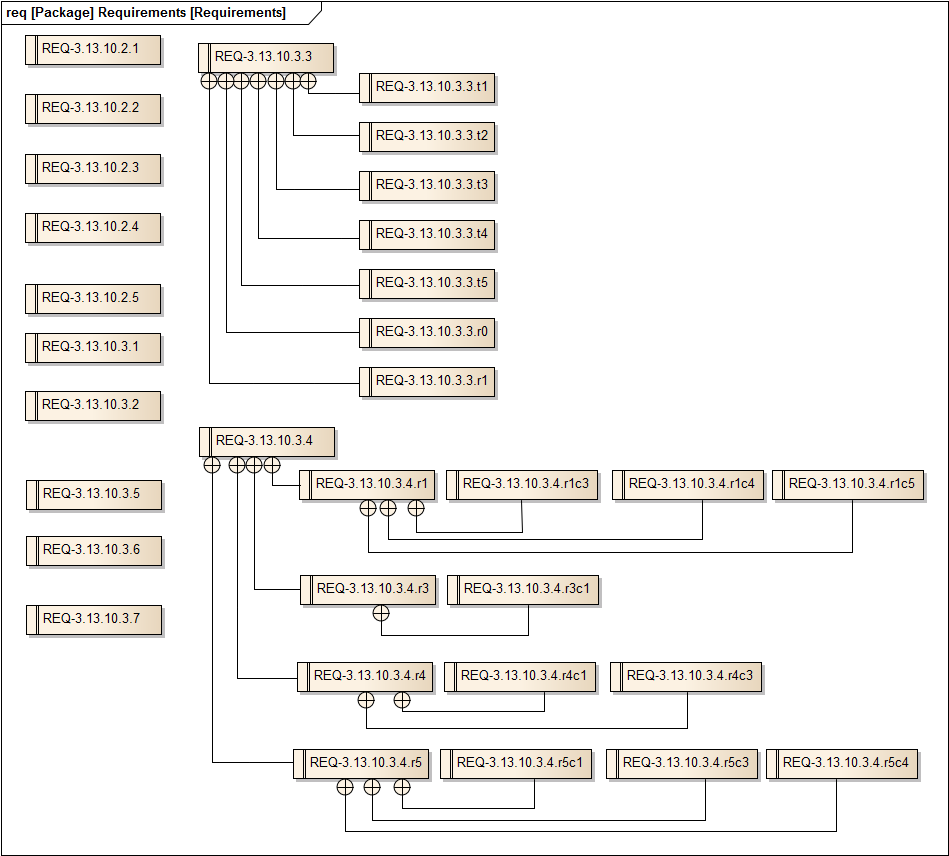
\includegraphics[width=1.3\textwidth]{Requirements.png}
%%\vspace*{-35mm}
\caption{System requirements diagram.}
 \label{fig:req}
 \end{figure}


 \begin{table}[htdp]
\caption{Requirements for the ceiling speed monitoring function.}
%\rule{\textwidth}{1pt}
\begin{center}
\footnotesize
\hspace*{-15mm}
\begin{tabular}{|c|p{130mm}|}
\hline\hline
{\bf id} & {\bf Description}
\\\hline\hline
REQ-3.13.10.2.1 & The train speed indicated to the driver shall be identical to the speed used for the speed monitoring (i.e. the estimated speed $\vest$).
\\\hline
REQ-3.13.10.2.2 & Once a Train Interface command (traction cut-off, service brake or emergency brake) is triggered, the on-board shall apply it until its corresponding revocation condition is met.
\\\hline
REQ-3.13.10.2.3 &
If there is no on-board interface with the service brake or if the use of the service brake command is not allowed by a National Value (only in Target speed monitoring),whenever a service brake command is specified, the emergency brake command shall be triggered instead.
\\\hline
REQ-3.13.10.2.4 &
The emergency brake command, which is triggered instead of the service brake command when an SBI supervision limit is exceeded, shall be revoked according to the requirements specified for the revocation of service brake command, unless the emergency brake command has been also triggered due to an EBI supervision limit. In such case, the condition for revoking the emergency brake command due to EBI supervision limit shall prevail.
\\\hline
REQ-3.13.10.2.5 &
The on-board shall revoke the Intervention status only when no brake command is applied by the speed and distance monitoring function.
\\\hline
%REQ-3.13.10.2.6 &
%In level 2/3: Train trip shall be initiated if the on-board equipment detects that the minimum safe front end has passed the EOA/LOA location.
%\\\hline
%REQ-3.13.10.2.7 &
%In Level 1: Train Trip shall be initiated if the on-board equipment detects that the minimum safe antenna position (calculated by subtracting distance between active Eurobalise antenna and the front end of the train from the min safe front end position) has passed the EOA/LOA location.
%\\\hline
REQ-3.13.10.3.1&
The on-board equipment shall display the permitted speed ($\vmax$).
\\\hline
REQ-3.13.10.3.2 &
When the supervision status is Overspeed, Warning or Intervention, the on-board equipment shall display the SBI speed (i.e. the FLOI speed; FLOI = First Line of Intervention).
\\\hline
REQ-3.13.10.3.3&
The on-board shall compare the estimated speed with the ceiling supervision limits defined in \cite[3.13.9.2]{ETCSSRS-Principles} and shall trigger/revoke commands to the train interface (service brake if implemented or emergency brake) and supervision statuses as described in Table~\ref{tab:five} (from~\cite[Table~5]{ETCSSRS-Principles}) and Table~\ref{tab:six} (from~\cite[Table~6]{ETCSSRS-Principles}).
\\\hline
REQ-3.13.10.3.4&
The on-board equipment shall execute the transitions between the different supervision statuses as described in Table~\ref{tab:seven} (see~\cite[4.6.1]{ETCSSRS-Principles} for details about the symbols). This table takes into account the order of precedence between the supervision statuses and the possible updates of the MRSP while in ceiling speed monitoring (e.g. when a TSR is revoked; TSR = Temporary Speed Restriction).
\\\hline
REQ-3.13.10.3.5&
When the speed and distance monitoring function becomes active and the ceiling speed monitoring is the first one entered, the triggering condition t1 defined in Table~\ref{tab:five} shall be checked in order to determine whether the Normal status applies. If it is not the case, the on-board shall immediately set the supervision status to the relevant value, applying a transition from the Normal status according to Table~\ref{tab:seven}.
\\\hline
REQ-3.13.10.3.6&
The Indication status is not used in ceiling speed monitoring. However, in case the ceiling speed monitoring is entered and the supervision status was previously set to Indication, the on-board equipment shall immediately execute one of the transitions from the Indication status, as described in Table~\ref{tab:seven}.
\\\hline
REQ-3.13.10.3.7&
The locations corresponding to a speed increase of the MRSP shall be supervised by the on-board equipment taking into account the min safe front end of the train.
\\\hline\hline
\end{tabular}
\normalsize
\end{center}
%\rule{\textwidth}{1pt}
\label{tab:req}
\end{table}%
 
\begin{table}[htdp]
\caption{Triggering of Train Interface commands and supervision statuses in ceiling speed monitoring (from~\cite[Table~5]{ETCSSRS-Principles}).}
\begin{center}
\footnotesize
\begin{tabular}{|l|c|l|c|l|}
\hline\hline
{\bf id} & {\bf TC} & {\bf Estimated speed} & {\bf TI} & {\bf SSE} 
\\\hline\hline
REQ-3.13.10.3.3.t1 & t1 & $\vest \le \vmax$ & --- & Normal Status
\\\hline
REQ-3.13.10.3.3.t2 & t2 & $\vest > \vmax$ & --- & Overspeed Status
\\\hline
REQ-3.13.10.3.3.t3 & t3 & $\vest > \vmax + \dvw$ & --- & Warning Status
\\\hline
REQ-3.13.10.3.3.t4 & t4 & $\vest > \vmax + \dvs$ & SB & Intervention Status
\\\hline
REQ-3.13.10.3.3.t5 & t5 & $\vest > \vmax + \dve$ & EB & Intervention Status  
\\\hline\hline
\end{tabular}
\normalsize
\end{center}

TC: trigger condition \newline
TI: command triggered on train interface to brakes \newline
SB: trigger service brake command (if available, otherwise trigger emergency brake)\newline
EB: trigger emergency brake command 
SSE: supervision status entered
\label{tab:five}
\end{table}%


\begin{table}[htdp]
\caption{Revocation of Train Interface commands and supervision statuses in ceiling speed monitoring (from~\cite[Table~6]{ETCSSRS-Principles}).}
\footnotesize
\begin{minipage}{\textwidth}
\begin{center}
\begin{tabular}{|l|c|c|c|p{4cm}|}
\hline\hline
{\bf id} & {\bf RC} & {\bf Estimated Speed} & {\bf TICR} & {\bf SSR}
\\\hline\hline
REQ-3.13.10.3.3.r0 & r0 & Standstill & EB & Intervention Status
\\\hline
REQ-3.13.10.3.3.r1 & r1 & $\vest \le \vmax$ & SB, EB\footnote{Only if $\text{allowRevokeEB} = 1$.} &
Indication Status \newline
Overspeed Status \newline
Warning Status \newline
Intervention Status (if SBI) \newline
Intervention Status (if EB and $\text{allowRevokeEB} = 1$)
\\\hline\hline
\end{tabular}
\end{center}
\end{minipage}
\normalsize

\medskip
RC: revocation condition \newline
TICR: command revoked on train interface to brakes \newline
SSR: supervision status revoked
\label{tab:six}
\end{table}%



\begin{table}[htdp]
\caption{Transitions between supervision statuses in ceiling speed
  monitoring (from~\cite[Table~7]{ETCSSRS-Principles}).}
\begin{center}
\footnotesize
%\begin{tabular}{|p{20mm}|p{20mm}|p{20mm}|p{20mm}|p{20mm}|}
\begin{tabular}{|c|c|c|c|c|}
\hline\hline
Normal Status & $< r1$ & $< r1$ & $< r1$ & $< r0,r1$
\\\hline
 & Indication Status & & & 
 \\\hline
 $t2 >$ & $t2 > $ & Overspeed Status & & 
 \\\hline
 $t3 >$ &  $t3 >$ &  $t3 >$ & Warning Status &
 \\\hline
 $t4,t5 >$ &  $t4,t5 >$ & $t4,t5 >$ & $t4,t5 >$ & Intervention Status
\\\hline\hline
\end{tabular}
\end{center}

\smallskip
 The
  sub-requirements IDs associated with each cell in the transition table
   are of the form  REQ-3.13.10.3.4.rX.cY where X and Y
  are the row and   column indexes, respectively. 
\normalsize
\label{tab:seven}
\end{table}%



% .......................................................................
%\newpage
\subsection{Behavioural Specification}
The behaviour of the ceiling speed monitor is modelled by the hierarchic state machine that is associated with the SUT block of Fig.~\ref{fig:sutcomposite} and displayed in Fig.~\ref{fig:csmsmtl} (top-level state machine) and Fig.~\ref{fig:csmsm} (lower-level state machine associated with composite state {\sf CSM\_ON}.


 \begin{figure}
 \centering
 \hspace*{-15mm}
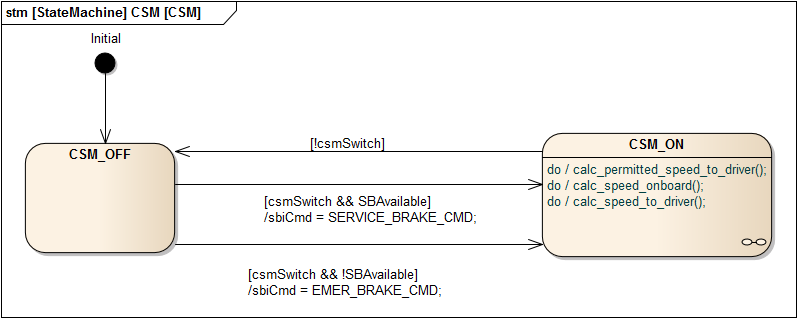
\includegraphics[width=1.2\textwidth]{CSM.png}
%%\vspace*{-35mm}
\caption{Ceiling speed monitoring -- top-level state machine.}
 \label{fig:csmsmtl}
 \end{figure}
 
 
 \begin{figure}
 \centering
\hspace*{-15mm}
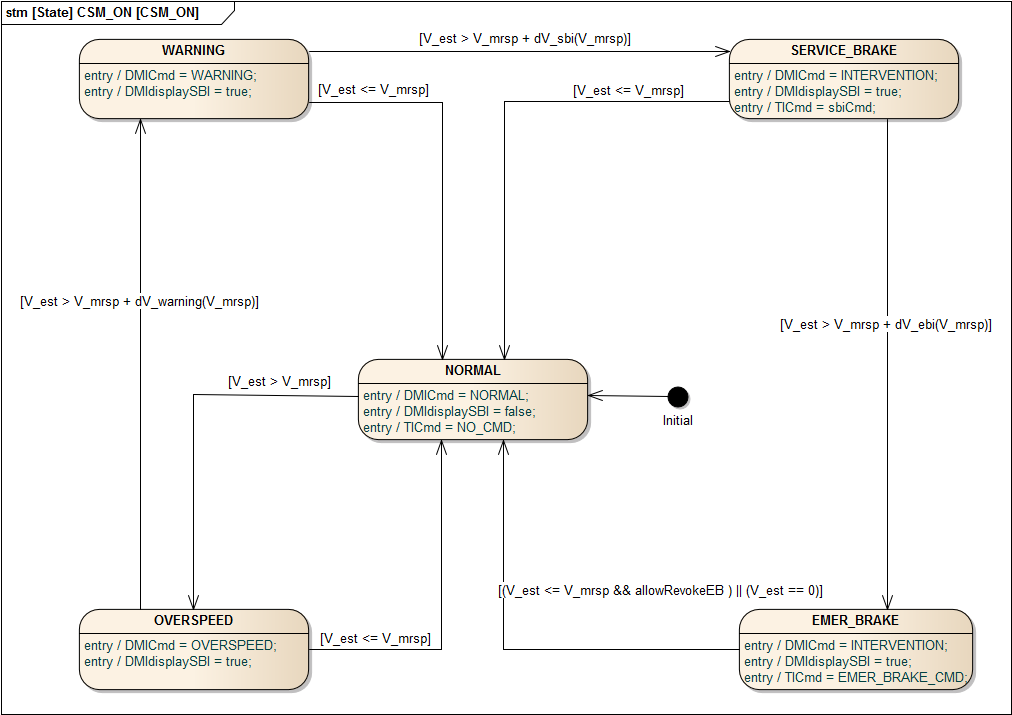
\includegraphics[width=1.2\textwidth]{CSM_ON_NO_FAILURE.png}
%%\vspace*{-35mm}
\caption{Ceiling speed monitoring state machine.}
 \label{fig:csmsm}
 \end{figure}



The top-level state machine controls activation and de-activation of the CSM. As soon as input 
variable $\csmsw$ on interface {\sf SnDMonitorIn} gets value 1, the CSM is activated, and it is de-activated when $\csmsw$ falls back to 0. On activation, the auxiliary variable $\sbicmd$ is set to EMER\_BRAKE\_CMD, if the input variable $\sbia$ carries value 0, indicating that no separate service brake can be used for slowing down the train, so that the emergency brake has to be used for this purpose. Conversely, when $\sbia = 1$, $\sbicmd$ is set to SERVICE\_BRAKE\_CMD. 


While in composite state {\sf CSM\_ON}, do actions are
executed as specified by operations\newline
 $\calcpstd$, $\calcsob$, and   $\calcstd$ 
introduced above. The effect of these
do actions is that variables $\pstd$, $\sob$, and $\std$ 
 are set consistently to the current values depending on $\vest$
and $\vmax$, respectively, as described above. The do-actions are executed whenever all state machine transitions are blocked, and the value of the left-hand side variable of the assignment performed by one of these operations differs from the valuation of the right-hand side expression. As a consequence, the necessary updates of these three output variables are executed in zero time after any input change.

Subordinate state machine {\sf CSM\_ON} specifies the detailed behaviour of the CSM. Its execution starts in basic state {\sf NORMAL}, where the `NORMAL' indication is displayed on the DMI and brakes are released ($\ticmd = \mathsf{NO\_CMD}$). When the speed increases above the maximal speed allowed ($\vest > \vmax$), the state machine transits to basic state {\sf OVERSPEED}, where the `OVERSPEED' indication is displayed to the train engine driver. If the train continues overspeeding until the warning threshold $\vmax + \dvw(\vmax)$ is exceeded, a transition
into the {\sf WARNING} state is performed, accompanied by an indication change on the DMI. Accelerating further until $\vest > \vmax + \dvs(\vmax)$ leads to a transition into basic state {\sf SERVICE\_BRAKE}, where either the service brake or the emergency brake is triggered, depending on the value stored before in variable $\sbicmd$. The DMI display changes to `INTERVENTION'. 

The intervention status is realised by two basic state machine states, {\sf SERVICE\_BRAKE} and
{\sf EMER\_BRAKE}. From {\sf SERVICE\_BRAKE} it is still possible to return to {\sf NORMAL}, as soon as the speed has been decreased below the overspeeding threshold. When the train, however, continues its acceleration until the emergency braking threshold has been exceeded ($\vest > \vmax+\dve(\vmax)$), basic state {\sf EMER\_BRAKE} is entered. From there, a state machine transition to {\sf NORMAL} is only possible if the train comes to a standstill, or if the national regulations (variable $\areb$)
allow to release the brakes as soon as overspeeding has stopped.

Observe that the run-to-completion semantics of state machines also allows for zero-time
 transitions from, for example, {\sf NORMAL} to {\sf EMER\_BRAKE}. If,
 while in basic state {\sf NORMAL},  the inputs change such that
 $\vest > \vmax+\dve(\vmax)$ becomes true\footnote{This would be an
   exceptional behaviour situation, caused, for example, by temporary
   unavailability of odometry data, so that a ``sudden jump'' of
   $\vest$ would be observed by the CSM.}, the state machine
 transition from {\sf NORMAL} to {\sf OVERSPEED} leads to a transient
 model state, because guard condition $\vest > \vmax+\dvw(\vmax)$ is already
 fulfilled, and the state machine transits to {\sf
   WARNING}. Similarly, guards $\vest > \vmax+\dvs(\vmax)$ and $\vest >
 \vmax+\dve(\vmax)$ also evaluate to true, so that the next quiescent state
 is reached in basic state {\sf EMER\_BRAKE}.
  Therefore  REQ-3.13.10.3.4.r5c1  which requires direct transitions from Normal status to Intervention status 
is fulfilled by the {\sf CSM\_ON} state machine: if the guard conditions have the appropriate valuations, the required target states can be reached in zero time, that is, in one observable EVC processing cycle. Analogously, the state machine fulfils requirements 
REQ-3.13.10.3.4.r5c2, REQ-3.13.10.3.4.r5c3, REQ-3.13.10.3.4.r4c1
without needing direct state machine transition arrows between the respective state machine states.


% .......................................................................
\newpage
\subsection{Requirements Tracing} 
SysML provides language elements for relating model elements to requirements, using the {\sf <<satisfy>>} relationship from model elements to requirements symbols in arbitrary SysML diagrams~\cite[Section~16]{SysML12}. Exploiting this language feature supports
\begin{itemize}
\item model validation, and
\item requirements-based testing.
\end{itemize}
In the former case, missing requirements can be detected if they
cannot be linked to structural or behavioural model elements in the
appropriate way. In latter case, execution traces through the model covering a
given structural or behavioural model element represent test cases
contributing to the verification of all requirements related to the
model element under consideration. 

%\begin{table}[htbp]
%\centering
%\includegraphics[height=\textheight]{requirements.pdf}
%\caption{\label{table:req-tracing} Requirements link to the SysML Elements}
%\end{table}


\begin{table}[htbp]
\caption{Requirements links to the SysML Elements}
\scriptsize
\begin{center}
\begin{tabular}{|r|l|l|}
\hline\hline
{\bf No.} & {\bf Requirement} & $\longleftarrow$ {\sf <<satisfy>>}
\\\hline\hline
1 &
REQ-3.13.10.2.1 & {\sf <<Composite State>>} {\sf CSM\_ON}  
\\\hline
2 &
REQ-3.13.10.2.2 & {\sf <<Transition>>} [{\sf EMER\_BRAKE} - {\sf NORMAL}]
\\ & &
{\sf <<Transition>>} [{\sf SERVICE\_BRAKE} - {\sf NORMAL}]
\\\hline
3 &
REQ-3.13.10.2.3 & {\sf <<Transition>>} [{\sf CSM\_OFF} - {\sf CSM\_ON}]
\\ & &
{\sf <<Basic State>>} {\sf SERVICE\_BRAKE}
\\ & &
{\sf <<Constraint>>} constraint\_03 
\\\hline
4 &
REQ-3.13.10.2.4 & {\sf <<Constraint>>} constraint\_02 
\\ & &
{\sf <<Transition>>} [{\sf EMER\_BRAKE} - {\sf NORMAL}]
\\ & &
{\sf <<Constraint>>} constraint\_01 
\\\hline
5 &
REQ-3.13.10.2.5 & {\sf <<Transition>>} [{\sf EMER\_BRAKE} - {\sf NORMAL}]
\\ & &
{\sf <<Transition>>} [{\sf SERVICE\_BRAKE} - {\sf NORMAL}]
\\\hline
6 &
REQ-3.13.10.3.1 & {\sf <<Submachine State>>} {\sf CSM\_ON}
\\\hline
7 &
REQ-3.13.10.3.2 & {\sf <<Basic State>>} {\sf OVERSPEED}  
\\ & &
{\sf <<Basic State>>} {\sf SERVICE\_BRAKE}  
\\ & &
{\sf <<Basic State>>} {\sf WARNING}  
\\ & &
{\sf <<Basic State>>} {\sf EMER\_BRAKE} 
\\\hline
8 &
REQ-3.13.10.3.3.r0 & {\sf <<Transition>>} [{\sf EMER\_BRAKE} - {\sf NORMAL}]
\\\hline
9 &
REQ-3.13.10.3.3.r1 & {\sf <<Transition>>} [{\sf OVERSPEED} - {\sf NORMAL}]
\\ & &
{\sf <<Transition>>} [{\sf SERVICE\_BRAKE} - {\sf NORMAL}]
\\ & &
{\sf <<Transition>>} [{\sf WARNING} - {\sf NORMAL}]
\\ & &
{\sf <<Transition>>} [{\sf EMER\_BRAKE} - {\sf NORMAL}]
\\\hline
10 &
REQ-3.13.10.3.3.t1 & {\sf <<Basic State>>} {\sf NORMAL}  
\\\hline
11 &
REQ-3.13.10.3.3.t2 & {\sf <<Basic State>>} {\sf OVERSPEED}  
\\\hline
12 &
REQ-3.13.10.3.3.t3 & {\sf <<Basic State>>} {\sf WARNING}  
\\\hline
13 &
REQ-3.13.10.3.3.t4 & {\sf <<Basic State>>} {\sf SERVICE\_BRAKE}  
\\\hline
14 &
REQ-3.13.10.3.3.t5 & {\sf <<Basic State>>} {\sf EMER\_BRAKE}  
\\\hline
15 &
REQ-3.13.10.3.4.r1c3 & {\sf <<Transition>>} [{\sf OVERSPEED} - {\sf NORMAL}]
\\\hline
16 &
REQ-3.13.10.3.4.r1c4 & {\sf <<Transition>>} [{\sf WARNING} - {\sf NORMAL}]
\\\hline
17 &
REQ-3.13.10.3.4.r1c5 & {\sf <<Transition>>} [{\sf EMER\_BRAKE} - {\sf NORMAL}]
\\ & &
{\sf <<Transition>>} [{\sf SERVICE\_BRAKE} - {\sf NORMAL}]
\\\hline
18 &
REQ-3.13.10.3.4.r3c1 & {\sf <<Transition>>} [{\sf NORMAL} - {\sf OVERSPEED}]
\\\hline
19 &
REQ-3.13.10.3.4.r4c1 & {\sf <<Constraint>>} constraint\_08 
\\\hline
20 &
REQ-3.13.10.3.4.r4c3 & {\sf <<Transition>>} [{\sf OVERSPEED} - {\sf WARNING}]
\\\hline
21 &
REQ-3.13.10.3.4.r5c1 & {\sf <<Constraint>>} constraint\_10 
\\ & &
{\sf <<Constraint>>} constraint\_09 
\\\hline
22 &
REQ-3.13.10.3.4.r5c3 & {\sf <<Constraint>>} constraint\_12 
\\ & &
{\sf <<Constraint>>} constraint\_11 
\\\hline
23 &
REQ-3.13.10.3.4.r5c4 & {\sf <<Transition>>} [{\sf WARNING} - {\sf SERVICE\_BRAKE}]
\\ & &
{\sf <<Transition>>} [{\sf SERVICE\_BRAKE} - {\sf EMER\_BRAKE}]
\\ & &
{\sf <<Constraint>>} constraint\_13 
\\\hline
24 &
REQ-3.13.10.3.5 & {\sf <<Constraint>>} constraint\_05 
\\ & &
{\sf <<Constraint>>} constraint\_06 
\\ & &
{\sf <<Constraint>>} constraint\_07 
\\ & &
{\sf <<Basic State>>} {\sf NORMAL} 
\\ & &
{\sf <<Constraint>>} constraint\_04 
\\\hline
25 &
REQ-3.13.10.3.6 & {\sf <<Constraint>>} constraint\_05 
\\ & &
{\sf <<Constraint>>} constraint\_06 
\\ & &
{\sf <<Constraint>>} constraint\_07 
\\ & &
{\sf <<Constraint>>} constraint\_04 

\\\hline\hline
\end{tabular}
\end{center}

\hspace*{15mm}
The constraints constraint\_01,\ldots,constraint\_13 are specified in Table~\ref{tab:constraints}.
\normalsize
\label{table:req-tracing} 
\end{table}

Tables \ref{table:req-tracing} associates 
the SysML elements with the requirements they satisfied.  ``Submachine
State'' and  ``Atomic State'' are the top-level and state machine
states, respectively. The ``Constraints" are the LTL formulas used to
relate the most complex requirements to execution traces as explained in the following paragraphs.
 

The complexity of {\sf <<satisfy>>} relations between structural or behavioural model elements depends on the complexity of the requirement and the way each requirement is reflected by the structural and behavioural model. Consider, for example (see Table~\ref{tab:req}), requirement  
\begin{quote}
REQ-3.13.10.2.1: The train speed indicated to the driver shall be identical to the speed used for the speed monitoring (i.e. the estimated speed $\vest$).
\end{quote}
Every model trace where the CSM is activated is suitable for verifying this requirement, because the DMI variable $\std$ is updated by the actual speed $\vest$ via operation $\calcstd$, whenever the ceiling speed monitor is active, that is, in composite state {\sf CSM\_ON}. Therefore 
{\sf CSM\_ON} is linked to REQ-3.13.10.2.1 by the {\sf <<satisfy>>} relation, as expressed
in Table~\ref{table:req-tracing}, row~1. 

 \begin{figure}
 \centering
\hspace*{-10mm}
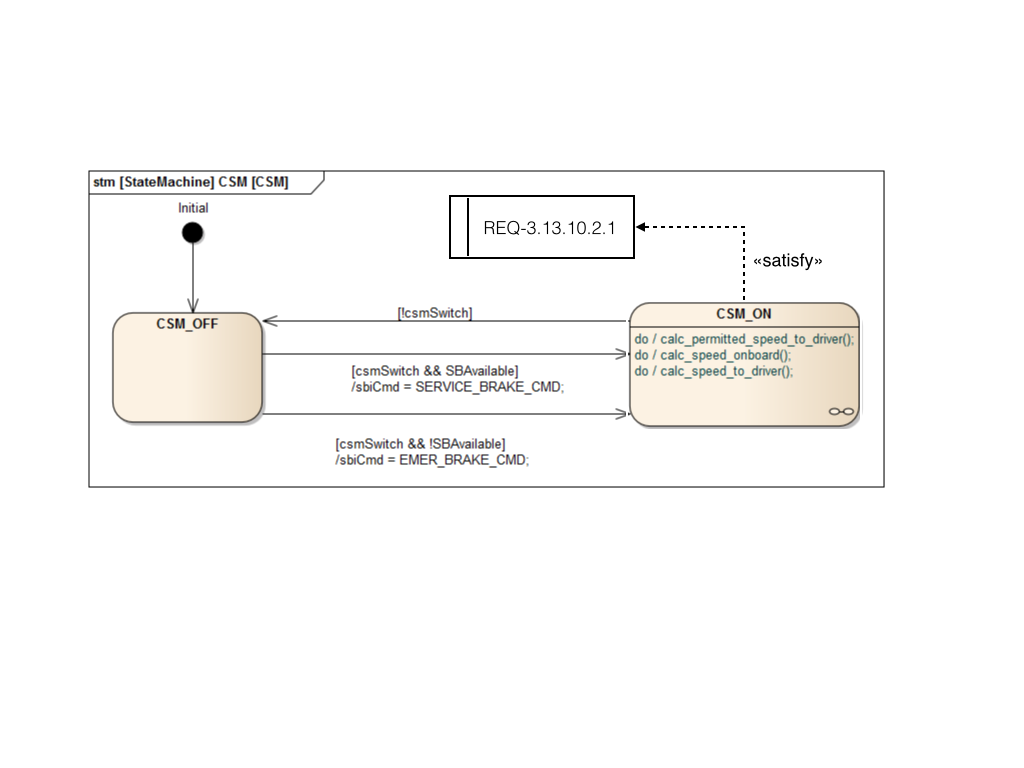
\includegraphics[width=1.2\textwidth]{CSM_ON_SATISFY.png}
\vspace*{-45mm}
\caption{Graphical representation of the {\sf <<satisfy>>} relation in a state machine diagram.}
 \label{fig:satisfy}
 \end{figure}


SysML also allows   to express traceability relationships in a graphical 
way, by drawing arrows from model elements to requirements as shown in Fig.~\ref{fig:satisfy}.
This technique, however, tends to clutter structural and behavioural diagrams as soon as more than a few requirements are involved. Therefore the tabular notation in Table~\ref{table:req-tracing} is preferable and supported by most state-of-the-art SysML modelling tools. 


A more complex case of requirements tracing presents itself if one or more transitions are related to a given requirement. This is the case for the requirement
\begin{quote}
REQ-3.13.10.2.2: Once a Train Interface command (traction cut-off, service brake or emergency brake) is triggered, the on-board shall apply it until its corresponding revocation condition is met.
\end{quote}
As modelled in Fig.~\ref{fig:csmsm}, we have two revocation conditions; one is reflected by the transition from basic state {\sf SERVICE\_BRAKE} to {\sf NORMAL}, the other from {\sf EMER\_BRAKE} to {\sf NORMAL}. Therefore both transitions are related to REQ-3.13.10.2.2, as specified in row~2 of Table~\ref{table:req-tracing}.



%For relating a transition to a requirement, an intermediate constraint is needed, specifying how the transition should be covered in order to check the requirement:
%\begin{itemize}
%\item Constraint keyword `TC' is used to specify that any variable valuation letting the guard condition evaluate to $\ist$ is suitable to verify the requirement.
%\item Constraint keyword `MC/DC' is used to specify that the transition needs to be performed several times, so that its guard condition is covered according to the Modified Condition/Decision Coverage (MC/DC) criterion, in order to verify the requirement.
%\end{itemize}
%The transition is connected to the constraint, and the constraint linked to the requirement by means of the {\sf <<satisfy>>} relationship. In this example, the MC/DC keyword is used in the constraint attached to the state machine transition from {\sf EMER\_BRAKE} to {\sf NORMAL}, because two variants of revocation conditions exist for this case, as specified in Table~\ref{tab:six}: for national value $\areb = 1$, we have to test that the emergency brake is already released when the estimated speed  is again below the maximal speed allowed ($\vest\le\vmax$);
%for $\areb = 0$, we have to test that the brakes are only released after the train has come to a standstill.


In the  most complex case we have to handle situations where requirements are reflected by traces visiting model state {\it vectors}\footnote{A model state vector consists of valuations of  inputs, outputs, and internal model variables, as well as of variable valuations indicating the basic state machine states currently active.} fulfilling certain constraints, and these model state vectors have to be visited by the traces in a specific order. Such a situation is reflected, for example, by 
\begin{quote}
REQ-3.13.10.3.4:
The on-board equipment shall execute the transitions between the different supervision statuses as described in Table~\ref{tab:seven} (see~\cite[4.6.1]{ETCSSRS-Principles} for details about the symbols). This table takes into account the order of precedence between the supervision statuses and the possible updates of the MRSP while in ceiling speed monitoring (e.g. when a TSR is revoked; TSR = Temporary Speed Restriction).
\end{quote}
This requirement   has been decomposed into atomic sub-requirements
REQ-3.13.10.3.4.r1c3, \ldots, REQ-3.13.10.3.4.r5c4, as explained in Section~\ref{sec:req}.
%REQ-3.13.10.3.4.r1c4, REQ-3.13.10.3.4.r1c5, REQ-3.13.10.3.4.r3c1, 
%REQ-3.13.10.3.4.r4c1, REQ-3.13.10.3.4.r4c3, REQ-3.13.10.3.4.r5c1, REQ-3.13.10.3.4.r5c3, REQ-3.13.10.3.4.r5c4, as explained in Section~\ref{sec:req}. 
Some of these sub-requirements are again 
reflected by transitions, as specified in rows 15, 16, 17, 18, and 20 of Table~\ref{table:req-tracing}. Requirement REQ-3.13.10.3.4.r5c1, however, specifies the possibility to directly transit from {\sf NORMAL} to {\sf SERVICE\_BRAKE} or {\sf EMER\_BRAKE}. This cannot be specified by simply linking a behavioural model element to the requirement, because we have avoided to draw direct state machine transitions from {\sf NORMAL} to {\sf SERVICE\_BRAKE} or {\sf EMER\_BRAKE}, since those transitions are implicitly realised by the run-to-completion semantics, as explained above.
Consider, for example, the zero-time transition
{\sf NORMAL} $\trans$ {\sf SERVICE\_BRAKE}. To cover this situation, we need to 
\begin{enumerate}
\item Enter   {\sf NORMAL} in a quiescent model state -- this is specified by 
$$[\mathsf{NORMAL} \wedge \vest \le \vmax]$$
\item Stay there until the speed exceeds $\vmax + \dvs(\vmax)$ but remains less or equal to $\vmax+\dve$.
\end{enumerate}
Formally this is expressed in LTL by 
\[
\begin{array}{l}
 \mathsf{Finally} ([\mathsf{NORMAL}\wedge \vest \le \vmax]  \wedge {}
 \\\tabf
 ([\mathsf{NORMAL}\wedge \vest \le \vmax]
 \\\tabf \ \
 \mathsf{Until}
 \\\tabf\
 [\mathsf{NORMAL}\wedge \vest > \vmax+\dvs(\vmax) \wedge {}
 \\\tabf \  \
 \vest \le \vmax+\dve(\vmax)]))
\end{array}
\]
This is expressed by constraint\_09 linked to REQ-3.13.10.3.4.r5c1 in Table~\ref{table:req-tracing} and specified in Table~\ref{tab:constraints}.
Similarly, covering the zero-time transition {\sf NORMAL} $\trans$ {\sf EMER\_BRAKE} requires a trace satisfying
\[
\begin{array}{l}
 \mathsf{Finally} ([\mathsf{NORMAL}\wedge \vest \le \vmax]  \wedge {}
 \\\tabf
 ([\mathsf{NORMAL}\wedge \vest \le \vmax]
 \\\tabf \ \
 \mathsf{Until}
 \\\tabf\
 [\mathsf{NORMAL}\wedge \vest > \vmax+\dve(\vmax)]))
\end{array}
\]
(this is specified as constraint\_10 in Table~\ref{tab:constraints}).
Similar constraints are specified for REQ-3.13.10.3.4.r4c1, REQ-3.13.10.3.4.r5c3, and 
REQ-3.13.10.3.4.r5c4, and for requirements REQ-3.13.10.3.5 and REQ-3.13.10.3.6.

 




\begin{table}[htdp]
\caption{Constraints related to complex requirements listed in Table~\ref{table:req-tracing}.}
\begin{center}
\scriptsize
\hspace*{-10mm}
\begin{tabular}{|l|p{12cm}|}
\hline\hline
{\sf <<Constraint>>} & {\bf LTL Formula}
\\\hline\hline
constraint\_01 & 
\parbox{120mm}{
\vspace*{1mm}
$\mathbf{Finally} [\mathsf{EMER\_BRAKE} \wedge \neg \sbia \wedge 
         \vest > 0 \wedge \vest \le  \vmax \wedge\neg  \areb]$ 
\vspace*{1mm}         
}
\\\hline
constraint\_02 &  
\parbox{120mm}{
\vspace*{1mm}
$\mathbf{Finally} [\mathsf{SERVICE\_BRAKE} \wedge\neg\sbia \wedge\vest\le\vmax]$
\vspace*{1mm}
}
\\\hline
constraint\_03 &  
\parbox{120mm}{
\vspace*{1mm}
$\mathbf{Finally} [\mathsf{SERVICE\_BRAKE} \wedge\neg\sbia\wedge \vest > \vmax + \dvs(\vmax) \wedge \vest \le \vmax + \dve(\vmax)]$
\vspace*{1mm}
}
\\\hline
constraint\_04 & 
\parbox{120mm}{
\vspace*{1mm}
$\mathbf{Finally} [\mathsf{CSM\_OFF} \wedge \csmsw \wedge \vest > \vmax  \wedge \vest \le \vmax + \dvw(\vmax) ]$
\vspace*{1mm}
} 
\\\hline
constraint\_05 &
\parbox{120mm}{
\vspace*{1mm}
$\mathbf{Finally} [\mathsf{CSM\_OFF} \wedge\csmsw \wedge \vest > \vmax + \dvw(\vmax) \wedge \vest\le\vmax+\dvs(\vmax) ]$
\vspace*{1mm}
}  
\\\hline
constraint\_06 & 
\parbox{120mm}{
\vspace*{1mm}
$\mathbf{Finally} [\mathsf{CSM\_OFF} \wedge\csmsw\wedge \vest > \vmax + \dvs(\vmax) \wedge \vest \le \vmax + \dve(\vmax) ]$
\vspace*{1mm}
} 
\\\hline
constraint\_07 &  
\parbox{120mm}{
\vspace*{1mm}
$\mathbf{Finally} [\mathsf{CSM\_OFF} \wedge\csmsw\wedge \vest > \vmax + \dve(\vmax) ]$
\vspace*{1mm}
}
\\\hline
constraint\_08 &  
\parbox{120mm}{
\vspace*{1mm}
$\mathbf{Finally} ([\mathsf{NORMAL} \wedge \vest\le\vmax] \wedge  
([\mathsf{NORMAL} \wedge  \vest\le\vmax]\ \mathbf{Until}\ [\mathsf{NORMAL} \wedge \vest > \vmax + \dvw(\vmax) \wedge \vest\le\vmax + \dvs(\vmax) ]))$
\vspace*{1mm}
}
\\\hline
constraint\_09 &  
\parbox{120mm}{
\vspace*{1mm}
$\mathbf{Finally} ([\mathsf{NORMAL} \wedge \vest\le\vmax] \wedge  
([\mathsf{NORMAL} \wedge  \vest\le\vmax]\ \mathbf{Until}\ [\mathsf{NORMAL} \wedge \vest > \vmax + \dvs(\vmax) \wedge \vest\le\vmax + \dve(\vmax) ]))$
\vspace*{1mm}
}
\\\hline
constraint\_10 &  
\parbox{120mm}{
\vspace*{1mm}
$\mathbf{Finally} ([\mathsf{NORMAL} \wedge \vest\le\vmax] \wedge  
([\mathsf{NORMAL} \wedge  \vest\le\vmax]\ \mathbf{Until}\ [\mathsf{NORMAL} \wedge \vest > \vmax + \dve(\vmax)]))$
\vspace*{1mm}
}
\\\hline
constraint\_11 &  
\parbox{120mm}{
\vspace*{1mm}
$\mathbf{Finally} ([\mathsf{OVERSPEED} \wedge \vest\le\vmax] \wedge  
([\mathsf{OVERSPEED} \wedge  \vest\le\vmax]\ \mathbf{Until}\ [\mathsf{OVERSPEED} \wedge \vest > \vmax + \dvs(\vmax) \wedge \vest\le\vmax + \dve(\vmax) ]))$
\vspace*{1mm}
}
\\\hline
constraint\_12 &  
\parbox{120mm}{
\vspace*{1mm}
$\mathbf{Finally} ([\mathsf{OVERSPEED} \wedge \vest\le\vmax] \wedge  
([\mathsf{OVERSPEED} \wedge  \vest\le\vmax]\ \mathbf{Until}\ [\mathsf{OVERSPEED} \wedge \vest > \vmax + \dve(\vmax)]))$
\vspace*{1mm}
}
\\\hline
constraint\_13 &  
\parbox{120mm}{
\vspace*{1mm}
$\mathbf{Finally} ([\mathsf{WARNING} \wedge \vest\le\vmax] \wedge  
([\mathsf{WARNING} \wedge  \vest\le\vmax]\ \mathbf{Until}\ [\mathsf{WARNING} \wedge \vest > \vmax + \dve(\vmax)]))$
\vspace*{1mm}
}
\\\hline\hline
\end{tabular}
\normalsize
\end{center}
\label{tab:constraints}
\end{table}%























